
%%%%%% We have discussed most of the commands in the class. Do practice them and the additional ones... 
%%% Please check the content of the pdf also as i have explained some commands.


\documentclass[10pt,a4paper]{report}
\usepackage[utf8]{inputenc}
\usepackage{amsmath}
\usepackage{amsfonts}
\usepackage{amssymb}
\usepackage{graphicx}
\title{Latex Notes }
\author{Asif Hamid}

\begin{document}
\maketitle
\newpage
\tableofcontents


\chapter{Introduction}
\section{Introduction to reinforcement learning}
\label{sec:introduction}
%%%%%% Observe how smartly the sections are labeled ...
\subsection{Definitions}
\label{sub:definitions}
Reinforcement learning is:
\begin{itemize}
    \item \textbf{agent-oriented learning:} learning by interacting with an environment
    \item \textbf{trial and error} only given delayed evaluative feedback
    \item \textbf{science of the mind} one which is neither natural science nor applied technology
\end{itemize}

Framework:
\begin{enumerate}
    \item agent percieves the \textbf{state} of the environment
    \item based on the state, it chooses an \textbf{action}
    \item the action gives the agent a \textbf{reward}
    \item a \textbf{policy} aims to maximize the agent's \textbf{long term expected reward}
\end{enumerate}
\section{Bandit}
\label{sec:bandit}

\subsection{Definition}
\label{sub:definition}

\textbf{One-armed bandit} Simplest RL problem
\begin{itemize}
    \item pull the lever
    \item get some reward
    \item choose the best lever!
\end{itemize}

\textbf{k-armed bandit} extends to $k$ arms
\begin{itemize}
    \item at every time step $t$, choose an action $A_t$ from $k$ possibilties
    \item recieve a reward $R_t$ dependent only on the action taken (i.i.d)
    \item $q_{a} = \mathbb{E} [R_t | A_t = a], \medskip \forall a \in {1, \dots k }$
\end{itemize}
%%%%%% \mathbb{•} command is used to insert the notation of a set...Try it

\vspace{2cm}
%%%%%
\begin{figure}[ht]
    \centering
    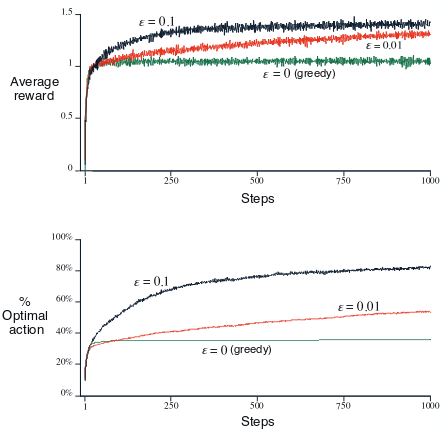
\includegraphics[width=0.9\linewidth]{epsilon_10arm.png}
    \caption{$\epsilon$-greedy methods on 10-arm bandit}
    \label{fig:Greedy}
\end{figure}
\section{Notes for latex class}
\textbf{Observe the two dollar sign for the command epsilon in the caption.} \\
Equation ;
\begin{equation}
\label{eq1}
	\begin{split}
	A & = \frac{\pi r^2}{2} \\
	 & = \frac{1}{2} \pi r^2
	\end{split}
\end{equation}
Note here the use of split env. Also the $\&$ operator which is used for alignment. If you can not understand this we will discuss this on monday.
Another equation example;
\begin{equation}
\label{FracEq}
f(x)=\frac{P(x)}{Q(x)} \\ \hspace{1cm} and \hspace{1cm}
	f(x)=\textstyle\frac{P(x)}{Q(x)}
\end{equation}
Note how I have used the command hspace in  (\ref{FracEq}) as we discussed in class on \textit{friday} to insert a gap for and.

The following equation is for the summation and integration, you can follow the same and adapt for different equations;
This is to use integration;
\begin{equation*}
y=\int_{a}^{b} x^2 \,dx
\end{equation*}
\begin{equation*}
z=\oint_V f(s) \,ds
\end{equation*}
Observe the use of $ \*$ as we discussed in the class. Also, try using \textbf{Split env} for the above two equations.

This one for summation;
\begin{equation}
\label{Sumeq}
\sum_{n=1}^{\infty} 2^{-n} = 1
\end{equation}
In (\ref{Sumeq}), analyse the use of underscores and curly braces. Try to understand this or we will discuss it in next class.
\par
We insert the limits with the equation env but we can also insert them in the text as Limit $\lim_{x\to\infty} f(x)$ inside text.


\chapter{Deep neural network}





%%%% this is my next section
\section{Motivation}
\label{Mot}
\subsubsection{Machine learning}
this is the first example.\\
\textbf{text text} this is the next section.
\begin{equation*}
y=3x
\end{equation*}

\begin{equation}
x=3x
\label{eq}
\end{equation}
In equation \ref{eq} we discussed  a linear system of the form $ x=2x \nleq y$ . \par 
%\hspace{2cm}

Observe the changes in the table code i have made. centering for center alignment, use of hspace and use of \textbf{Table env} for caption and labeling. \textbf{Tabular env} is for inserting table only. I forgot to mention this in the class.
\begin{table}

\label{Tab1}
\caption{List of prices}
\centering
\hspace{2cm}

\begin{tabular}{|c|c|c|c|c|}
\hline 
First & second & third & fourth & fifth \\ 
\hline 
• & • & • & • & • \\ [0.5cm]
\hline 
• & • & • & • & • \\ 
\hline 
• & • & • & • & • \\ 
\hline 
• & • & • & • & • \\ 
\hline 
\end{tabular} 
\end{table}











In section \ref{Mot} we discussed the motivation for the report.
\begin{enumerate}
\item Detergent
\item Rice.\label{Ric}
\item Dal.
\item fruits.

\end{enumerate}
The items have following prices;
\begin{itemize}
\item Price of item-\ref{Ric} is Rs 70/kg.
\item 60
\item 20
\end{itemize}
\hspace{5cm} The next section discusses further prices.










%
%\begin{figure}[b!]
%\includegraphics[width=0.5\linewidth]{logo}
%\caption{example figure of lecture 1}
%\label{fig1}
%\end{figure}




In Figure \ref{fig:Greedy} we have shown the results.








This is an example of latex.
\end{document}